\documentclass[twoside]{book}

% Packages required by doxygen
\usepackage{fixltx2e}
\usepackage{calc}
\usepackage{doxygen}
\usepackage[export]{adjustbox} % also loads graphicx
\usepackage{graphicx}
\usepackage[utf8]{inputenc}
\usepackage{makeidx}
\usepackage{multicol}
\usepackage{multirow}
\PassOptionsToPackage{warn}{textcomp}
\usepackage{textcomp}
\usepackage[nointegrals]{wasysym}
\usepackage[table]{xcolor}

% Font selection
\usepackage[T1]{fontenc}
\usepackage[scaled=.90]{helvet}
\usepackage{courier}
\usepackage{amssymb}
\usepackage{sectsty}
\renewcommand{\familydefault}{\sfdefault}
\allsectionsfont{%
  \fontseries{bc}\selectfont%
  \color{darkgray}%
}
\renewcommand{\DoxyLabelFont}{%
  \fontseries{bc}\selectfont%
  \color{darkgray}%
}
\newcommand{\+}{\discretionary{\mbox{\scriptsize$\hookleftarrow$}}{}{}}

% Page & text layout
\usepackage{geometry}
\geometry{%
  a4paper,%
  top=2.5cm,%
  bottom=2.5cm,%
  left=2.5cm,%
  right=2.5cm%
}
\tolerance=750
\hfuzz=15pt
\hbadness=750
\setlength{\emergencystretch}{15pt}
\setlength{\parindent}{0cm}
\setlength{\parskip}{3ex plus 2ex minus 2ex}
\makeatletter
\renewcommand{\paragraph}{%
  \@startsection{paragraph}{4}{0ex}{-1.0ex}{1.0ex}{%
    \normalfont\normalsize\bfseries\SS@parafont%
  }%
}
\renewcommand{\subparagraph}{%
  \@startsection{subparagraph}{5}{0ex}{-1.0ex}{1.0ex}{%
    \normalfont\normalsize\bfseries\SS@subparafont%
  }%
}
\makeatother

% Headers & footers
\usepackage{fancyhdr}
\pagestyle{fancyplain}
\fancyhead[LE]{\fancyplain{}{\bfseries\thepage}}
\fancyhead[CE]{\fancyplain{}{}}
\fancyhead[RE]{\fancyplain{}{\bfseries\leftmark}}
\fancyhead[LO]{\fancyplain{}{\bfseries\rightmark}}
\fancyhead[CO]{\fancyplain{}{}}
\fancyhead[RO]{\fancyplain{}{\bfseries\thepage}}
\fancyfoot[LE]{\fancyplain{}{}}
\fancyfoot[CE]{\fancyplain{}{}}
\fancyfoot[RE]{\fancyplain{}{\bfseries\scriptsize Generated by Doxygen }}
\fancyfoot[LO]{\fancyplain{}{\bfseries\scriptsize Generated by Doxygen }}
\fancyfoot[CO]{\fancyplain{}{}}
\fancyfoot[RO]{\fancyplain{}{}}
\renewcommand{\footrulewidth}{0.4pt}
\renewcommand{\chaptermark}[1]{%
  \markboth{#1}{}%
}
\renewcommand{\sectionmark}[1]{%
  \markright{\thesection\ #1}%
}

% Indices & bibliography
\usepackage{natbib}
\usepackage[titles]{tocloft}
\setcounter{tocdepth}{3}
\setcounter{secnumdepth}{5}
\makeindex

% Hyperlinks (required, but should be loaded last)
\usepackage{ifpdf}
\ifpdf
  \usepackage[pdftex,pagebackref=true]{hyperref}
\else
  \usepackage[ps2pdf,pagebackref=true]{hyperref}
\fi
\hypersetup{%
  colorlinks=true,%
  linkcolor=blue,%
  citecolor=blue,%
  unicode%
}

% Custom commands
\newcommand{\clearemptydoublepage}{%
  \newpage{\pagestyle{empty}\cleardoublepage}%
}

\usepackage{caption}
\captionsetup{labelsep=space,justification=centering,font={bf},singlelinecheck=off,skip=4pt,position=top}

%===== C O N T E N T S =====

\begin{document}

% Titlepage & ToC
\hypersetup{pageanchor=false,
             bookmarksnumbered=true,
             pdfencoding=unicode
            }
\pagenumbering{roman}
\begin{titlepage}
\vspace*{7cm}
\begin{center}%
{\Large Cloud\+Core\+Interface }\\
\vspace*{1cm}
{\large Generated by Doxygen 1.8.11}\\
\end{center}
\end{titlepage}
\clearemptydoublepage
\tableofcontents
\clearemptydoublepage
\pagenumbering{arabic}
\hypersetup{pageanchor=true}

%--- Begin generated contents ---
\chapter{R\+E\+A\+D\+ME}
\label{md_README}
\hypertarget{md_README}{}
\href{https://api.travis-ci.org/symbiote-h2020/CloudCoreInterface}{\tt } \href{https://codecov.io/github/symbiote-h2020/CloudCoreInterface}{\tt }

\section*{Cloud\+Core\+Interface}
\chapter{Class Index}
\section{Class List}
Here are the classes, structs, unions and interfaces with brief descriptions\+:\begin{DoxyCompactList}
\item\contentsline{section}{\hyperlink{classeu_1_1h2020_1_1symbiote_1_1CloudCoreInterfaceApplication}{eu.\+h2020.\+symbiote.\+Cloud\+Core\+Interface\+Application} }{\pageref{classeu_1_1h2020_1_1symbiote_1_1CloudCoreInterfaceApplication}}{}
\item\contentsline{section}{\hyperlink{classeu_1_1h2020_1_1symbiote_1_1controllers_1_1CloudCoreInterfaceController}{eu.\+h2020.\+symbiote.\+controllers.\+Cloud\+Core\+Interface\+Controller} }{\pageref{classeu_1_1h2020_1_1symbiote_1_1controllers_1_1CloudCoreInterfaceController}}{}
\item\contentsline{section}{\hyperlink{classeu_1_1h2020_1_1symbiote_1_1communication_1_1RabbitManager}{eu.\+h2020.\+symbiote.\+communication.\+Rabbit\+Manager} }{\pageref{classeu_1_1h2020_1_1symbiote_1_1communication_1_1RabbitManager}}{}
\end{DoxyCompactList}

\chapter{Class Documentation}
\hypertarget{classeu_1_1h2020_1_1symbiote_1_1CloudCoreInterfaceApplication}{}\section{eu.\+h2020.\+symbiote.\+Cloud\+Core\+Interface\+Application Class Reference}
\label{classeu_1_1h2020_1_1symbiote_1_1CloudCoreInterfaceApplication}\index{eu.\+h2020.\+symbiote.\+Cloud\+Core\+Interface\+Application@{eu.\+h2020.\+symbiote.\+Cloud\+Core\+Interface\+Application}}


Collaboration diagram for eu.\+h2020.\+symbiote.\+Cloud\+Core\+Interface\+Application\+:\nopagebreak
\begin{figure}[H]
\begin{center}
\leavevmode
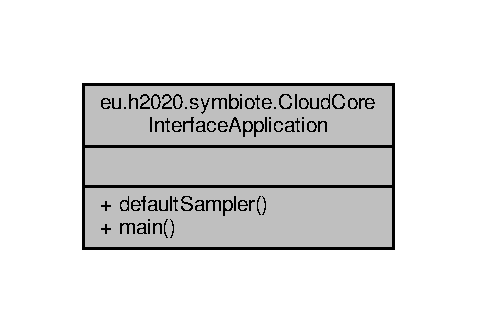
\includegraphics[width=229pt]{classeu_1_1h2020_1_1symbiote_1_1CloudCoreInterfaceApplication__coll__graph}
\end{center}
\end{figure}
\subsection*{Classes}
\begin{DoxyCompactItemize}
\item 
class {\bfseries C\+LR}
\end{DoxyCompactItemize}
\subsection*{Public Member Functions}
\begin{DoxyCompactItemize}
\item 
\mbox{\Hypertarget{classeu_1_1h2020_1_1symbiote_1_1CloudCoreInterfaceApplication_a12ccc55e03aebfb165dd037cefc9bb78}\label{classeu_1_1h2020_1_1symbiote_1_1CloudCoreInterfaceApplication_a12ccc55e03aebfb165dd037cefc9bb78}} 
Always\+Sampler {\bfseries default\+Sampler} ()
\end{DoxyCompactItemize}
\subsection*{Static Public Member Functions}
\begin{DoxyCompactItemize}
\item 
\mbox{\Hypertarget{classeu_1_1h2020_1_1symbiote_1_1CloudCoreInterfaceApplication_a19264807749c01cd7938facb44578f43}\label{classeu_1_1h2020_1_1symbiote_1_1CloudCoreInterfaceApplication_a19264807749c01cd7938facb44578f43}} 
static void {\bfseries main} (String\mbox{[}$\,$\mbox{]} args)
\end{DoxyCompactItemize}


\subsection{Detailed Description}
Cloud-\/\+Core Interface module\textquotesingle{}s entry point. 

Cloud-\/\+Core Interface is a southbound interface for accessing symb\+Io\+Te platform. It allows platform owners to register their resources. 

The documentation for this class was generated from the following file\+:\begin{DoxyCompactItemize}
\item 
src/main/java/eu/h2020/symbiote/Cloud\+Core\+Interface\+Application.\+java\end{DoxyCompactItemize}

\hypertarget{classeu_1_1h2020_1_1symbiote_1_1controllers_1_1CloudCoreInterfaceController}{}\section{eu.\+h2020.\+symbiote.\+controllers.\+Cloud\+Core\+Interface\+Controller Class Reference}
\label{classeu_1_1h2020_1_1symbiote_1_1controllers_1_1CloudCoreInterfaceController}\index{eu.\+h2020.\+symbiote.\+controllers.\+Cloud\+Core\+Interface\+Controller@{eu.\+h2020.\+symbiote.\+controllers.\+Cloud\+Core\+Interface\+Controller}}


Collaboration diagram for eu.\+h2020.\+symbiote.\+controllers.\+Cloud\+Core\+Interface\+Controller\+:
\nopagebreak
\begin{figure}[H]
\begin{center}
\leavevmode
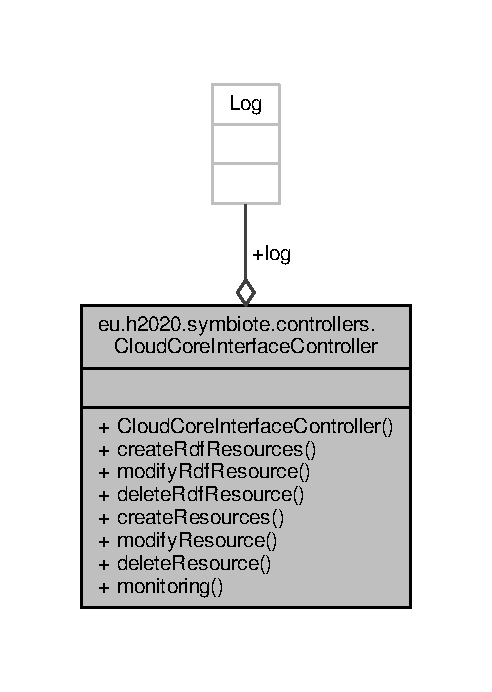
\includegraphics[width=238pt]{classeu_1_1h2020_1_1symbiote_1_1controllers_1_1CloudCoreInterfaceController__coll__graph}
\end{center}
\end{figure}
\subsection*{Public Member Functions}
\begin{DoxyCompactItemize}
\item 
\hyperlink{classeu_1_1h2020_1_1symbiote_1_1controllers_1_1CloudCoreInterfaceController_a19222abf4496aac62c037451b02c7f31}{Cloud\+Core\+Interface\+Controller} (\hyperlink{classeu_1_1h2020_1_1symbiote_1_1communication_1_1RabbitManager}{Rabbit\+Manager} rabbit\+Manager)
\item 
Response\+Entity$<$?$>$ \hyperlink{classeu_1_1h2020_1_1symbiote_1_1controllers_1_1CloudCoreInterfaceController_a86e93a8ba38be222f570d850ca2cfed0}{create\+Rdf\+Resources} (@Path\+Variable(\char`\"{}platform\+Id\char`\"{}) String platform\+Id,@Request\+Body String rdf\+Resources)
\item 
Response\+Entity$<$?$>$ \hyperlink{classeu_1_1h2020_1_1symbiote_1_1controllers_1_1CloudCoreInterfaceController_add9d780c27d48dfce1c84537b3e2963e}{modify\+Rdf\+Resource} (@Path\+Variable(\char`\"{}platform\+Id\char`\"{}) String platform\+Id,@Path\+Variable(\char`\"{}resource\+Id\char`\"{}) String resource\+Id,@Request\+Body String rdf\+Resources)
\item 
Response\+Entity$<$?$>$ \hyperlink{classeu_1_1h2020_1_1symbiote_1_1controllers_1_1CloudCoreInterfaceController_a1470a53850a203a85db8f0b93d18c362}{delete\+Rdf\+Resource} (@Path\+Variable(\char`\"{}platform\+Id\char`\"{}) String platform\+Id,@Path\+Variable(\char`\"{}resource\+Id\char`\"{}) String resource\+Id)
\item 
Response\+Entity$<$?$>$ \hyperlink{classeu_1_1h2020_1_1symbiote_1_1controllers_1_1CloudCoreInterfaceController_a9519d747900350a3e05f859a37c53780}{create\+Resources} (@Path\+Variable(\char`\"{}platform\+Id\char`\"{}) String platform\+Id,@Request\+Body \hyperlink{classeu_1_1h2020_1_1symbiote_1_1model_1_1Resource}{Resource} resource)
\item 
Response\+Entity$<$?$>$ \hyperlink{classeu_1_1h2020_1_1symbiote_1_1controllers_1_1CloudCoreInterfaceController_abb8609ab8c4a98d633a12d137e48ece8}{modify\+Resource} (@Path\+Variable(\char`\"{}platform\+Id\char`\"{}) String platform\+Id,@Path\+Variable(\char`\"{}resource\+Id\char`\"{}) String resource\+Id,@Request\+Body \hyperlink{classeu_1_1h2020_1_1symbiote_1_1model_1_1Resource}{Resource} resource)
\item 
Response\+Entity$<$?$>$ \hyperlink{classeu_1_1h2020_1_1symbiote_1_1controllers_1_1CloudCoreInterfaceController_a9697cf03798b509844d2dc675c50e463}{delete\+Resource} (@Path\+Variable(\char`\"{}platform\+Id\char`\"{}) String platform\+Id,@Path\+Variable(\char`\"{}resource\+Id\char`\"{}) String resource\+Id)
\end{DoxyCompactItemize}
\subsection*{Static Public Attributes}
\begin{DoxyCompactItemize}
\item 
static Log {\bfseries log} = Log\+Factory.\+get\+Log(Cloud\+Core\+Interface\+Controller.\+class)\hypertarget{classeu_1_1h2020_1_1symbiote_1_1controllers_1_1CloudCoreInterfaceController_a984b8c1127a0c63545f1633b53ab8b00}{}\label{classeu_1_1h2020_1_1symbiote_1_1controllers_1_1CloudCoreInterfaceController_a984b8c1127a0c63545f1633b53ab8b00}

\end{DoxyCompactItemize}


\subsection{Detailed Description}
Class defining all R\+E\+ST endpoints. 

Cloud\+Core\+Interface, as the name suggests, is just an interface, therefore it forwards all requests to modules responsible for handling them via Rabbit\+MQ. 

\subsection{Constructor \& Destructor Documentation}
\index{eu\+::h2020\+::symbiote\+::controllers\+::\+Cloud\+Core\+Interface\+Controller@{eu\+::h2020\+::symbiote\+::controllers\+::\+Cloud\+Core\+Interface\+Controller}!Cloud\+Core\+Interface\+Controller@{Cloud\+Core\+Interface\+Controller}}
\index{Cloud\+Core\+Interface\+Controller@{Cloud\+Core\+Interface\+Controller}!eu\+::h2020\+::symbiote\+::controllers\+::\+Cloud\+Core\+Interface\+Controller@{eu\+::h2020\+::symbiote\+::controllers\+::\+Cloud\+Core\+Interface\+Controller}}
\subsubsection[{\texorpdfstring{Cloud\+Core\+Interface\+Controller(\+Rabbit\+Manager rabbit\+Manager)}{CloudCoreInterfaceController(RabbitManager rabbitManager)}}]{\setlength{\rightskip}{0pt plus 5cm}eu.\+h2020.\+symbiote.\+controllers.\+Cloud\+Core\+Interface\+Controller.\+Cloud\+Core\+Interface\+Controller (
\begin{DoxyParamCaption}
\item[{{\bf Rabbit\+Manager}}]{rabbit\+Manager}
\end{DoxyParamCaption}
)}\hypertarget{classeu_1_1h2020_1_1symbiote_1_1controllers_1_1CloudCoreInterfaceController_a19222abf4496aac62c037451b02c7f31}{}\label{classeu_1_1h2020_1_1symbiote_1_1controllers_1_1CloudCoreInterfaceController_a19222abf4496aac62c037451b02c7f31}
Class constructor which autowires Rabbit\+Manager bean.


\begin{DoxyParams}{Parameters}
{\em rabbit\+Manager} & Rabbit\+Manager bean \\
\hline
\end{DoxyParams}


\subsection{Member Function Documentation}
\index{eu\+::h2020\+::symbiote\+::controllers\+::\+Cloud\+Core\+Interface\+Controller@{eu\+::h2020\+::symbiote\+::controllers\+::\+Cloud\+Core\+Interface\+Controller}!create\+Rdf\+Resources@{create\+Rdf\+Resources}}
\index{create\+Rdf\+Resources@{create\+Rdf\+Resources}!eu\+::h2020\+::symbiote\+::controllers\+::\+Cloud\+Core\+Interface\+Controller@{eu\+::h2020\+::symbiote\+::controllers\+::\+Cloud\+Core\+Interface\+Controller}}
\subsubsection[{\texorpdfstring{create\+Rdf\+Resources("@Path\+Variable(""platform\+Id"") String platform\+Id,"@Request\+Body String rdf\+Resources)}{createRdfResources(@PathVariable("platformId") String platformId,@RequestBody String rdfResources)}}]{\setlength{\rightskip}{0pt plus 5cm}Response\+Entity$<$?$>$ eu.\+h2020.\+symbiote.\+controllers.\+Cloud\+Core\+Interface\+Controller.\+create\+Rdf\+Resources (
\begin{DoxyParamCaption}
\item[{@Path\+Variable(\char`\"{}platform\+Id\char`\"{}) String}]{platform\+Id, }
\item[{@Request\+Body String}]{rdf\+Resources}
\end{DoxyParamCaption}
)}\hypertarget{classeu_1_1h2020_1_1symbiote_1_1controllers_1_1CloudCoreInterfaceController_a86e93a8ba38be222f570d850ca2cfed0}{}\label{classeu_1_1h2020_1_1symbiote_1_1controllers_1_1CloudCoreInterfaceController_a86e93a8ba38be222f570d850ca2cfed0}
Endpoint for creating resource using R\+DF description. 

Currently not implemented. \index{eu\+::h2020\+::symbiote\+::controllers\+::\+Cloud\+Core\+Interface\+Controller@{eu\+::h2020\+::symbiote\+::controllers\+::\+Cloud\+Core\+Interface\+Controller}!create\+Resources@{create\+Resources}}
\index{create\+Resources@{create\+Resources}!eu\+::h2020\+::symbiote\+::controllers\+::\+Cloud\+Core\+Interface\+Controller@{eu\+::h2020\+::symbiote\+::controllers\+::\+Cloud\+Core\+Interface\+Controller}}
\subsubsection[{\texorpdfstring{create\+Resources("@Path\+Variable(""platform\+Id"") String platform\+Id,"@Request\+Body Resource resource)}{createResources(@PathVariable("platformId") String platformId,@RequestBody Resource resource)}}]{\setlength{\rightskip}{0pt plus 5cm}Response\+Entity$<$?$>$ eu.\+h2020.\+symbiote.\+controllers.\+Cloud\+Core\+Interface\+Controller.\+create\+Resources (
\begin{DoxyParamCaption}
\item[{@Path\+Variable(\char`\"{}platform\+Id\char`\"{}) String}]{platform\+Id, }
\item[{@Request\+Body {\bf Resource}}]{resource}
\end{DoxyParamCaption}
)}\hypertarget{classeu_1_1h2020_1_1symbiote_1_1controllers_1_1CloudCoreInterfaceController_a9519d747900350a3e05f859a37c53780}{}\label{classeu_1_1h2020_1_1symbiote_1_1controllers_1_1CloudCoreInterfaceController_a9519d747900350a3e05f859a37c53780}
Endpoint for creating resource using J\+S\+ON description.


\begin{DoxyParams}{Parameters}
{\em platform\+Id} & ID of a platform that resource belongs to; if platform ID is specified in Resource body object, it will be overwritten by path parameter \\
\hline
{\em resource} & resource that is to be registered \\
\hline
\end{DoxyParams}
\begin{DoxyReturn}{Returns}
created resource (with resource\+Id filled) or null along with appropriate error H\+T\+TP status code 
\end{DoxyReturn}
\index{eu\+::h2020\+::symbiote\+::controllers\+::\+Cloud\+Core\+Interface\+Controller@{eu\+::h2020\+::symbiote\+::controllers\+::\+Cloud\+Core\+Interface\+Controller}!delete\+Rdf\+Resource@{delete\+Rdf\+Resource}}
\index{delete\+Rdf\+Resource@{delete\+Rdf\+Resource}!eu\+::h2020\+::symbiote\+::controllers\+::\+Cloud\+Core\+Interface\+Controller@{eu\+::h2020\+::symbiote\+::controllers\+::\+Cloud\+Core\+Interface\+Controller}}
\subsubsection[{\texorpdfstring{delete\+Rdf\+Resource("@Path\+Variable(""platform\+Id"") String platform\+Id,"@Path\+Variable(""resource\+Id"") String resource\+Id)}{deleteRdfResource(@PathVariable("platformId") String platformId,@PathVariable("resourceId") String resourceId)}}]{\setlength{\rightskip}{0pt plus 5cm}Response\+Entity$<$?$>$ eu.\+h2020.\+symbiote.\+controllers.\+Cloud\+Core\+Interface\+Controller.\+delete\+Rdf\+Resource (
\begin{DoxyParamCaption}
\item[{@Path\+Variable(\char`\"{}platform\+Id\char`\"{}) String}]{platform\+Id, }
\item[{@Path\+Variable(\char`\"{}resource\+Id\char`\"{}) String}]{resource\+Id}
\end{DoxyParamCaption}
)}\hypertarget{classeu_1_1h2020_1_1symbiote_1_1controllers_1_1CloudCoreInterfaceController_a1470a53850a203a85db8f0b93d18c362}{}\label{classeu_1_1h2020_1_1symbiote_1_1controllers_1_1CloudCoreInterfaceController_a1470a53850a203a85db8f0b93d18c362}
Endpoint for deleting resource using R\+DF description. 

Currently not implemented. \index{eu\+::h2020\+::symbiote\+::controllers\+::\+Cloud\+Core\+Interface\+Controller@{eu\+::h2020\+::symbiote\+::controllers\+::\+Cloud\+Core\+Interface\+Controller}!delete\+Resource@{delete\+Resource}}
\index{delete\+Resource@{delete\+Resource}!eu\+::h2020\+::symbiote\+::controllers\+::\+Cloud\+Core\+Interface\+Controller@{eu\+::h2020\+::symbiote\+::controllers\+::\+Cloud\+Core\+Interface\+Controller}}
\subsubsection[{\texorpdfstring{delete\+Resource("@Path\+Variable(""platform\+Id"") String platform\+Id,"@Path\+Variable(""resource\+Id"") String resource\+Id)}{deleteResource(@PathVariable("platformId") String platformId,@PathVariable("resourceId") String resourceId)}}]{\setlength{\rightskip}{0pt plus 5cm}Response\+Entity$<$?$>$ eu.\+h2020.\+symbiote.\+controllers.\+Cloud\+Core\+Interface\+Controller.\+delete\+Resource (
\begin{DoxyParamCaption}
\item[{@Path\+Variable(\char`\"{}platform\+Id\char`\"{}) String}]{platform\+Id, }
\item[{@Path\+Variable(\char`\"{}resource\+Id\char`\"{}) String}]{resource\+Id}
\end{DoxyParamCaption}
)}\hypertarget{classeu_1_1h2020_1_1symbiote_1_1controllers_1_1CloudCoreInterfaceController_a9697cf03798b509844d2dc675c50e463}{}\label{classeu_1_1h2020_1_1symbiote_1_1controllers_1_1CloudCoreInterfaceController_a9697cf03798b509844d2dc675c50e463}
Endpoint for removing resource using J\+S\+ON description.


\begin{DoxyParams}{Parameters}
{\em platform\+Id} & ID of a platform that resource belongs to \\
\hline
{\em resource\+Id} & ID of a resource to remove \\
\hline
\end{DoxyParams}
\begin{DoxyReturn}{Returns}
empty body with appropriate operation H\+T\+TP status code 
\end{DoxyReturn}
\index{eu\+::h2020\+::symbiote\+::controllers\+::\+Cloud\+Core\+Interface\+Controller@{eu\+::h2020\+::symbiote\+::controllers\+::\+Cloud\+Core\+Interface\+Controller}!modify\+Rdf\+Resource@{modify\+Rdf\+Resource}}
\index{modify\+Rdf\+Resource@{modify\+Rdf\+Resource}!eu\+::h2020\+::symbiote\+::controllers\+::\+Cloud\+Core\+Interface\+Controller@{eu\+::h2020\+::symbiote\+::controllers\+::\+Cloud\+Core\+Interface\+Controller}}
\subsubsection[{\texorpdfstring{modify\+Rdf\+Resource("@Path\+Variable(""platform\+Id"") String platform\+Id,"@Path\+Variable(""resource\+Id"") String resource\+Id,"@Request\+Body String rdf\+Resources)}{modifyRdfResource(@PathVariable("platformId") String platformId,@PathVariable("resourceId") String resourceId,@RequestBody String rdfResources)}}]{\setlength{\rightskip}{0pt plus 5cm}Response\+Entity$<$?$>$ eu.\+h2020.\+symbiote.\+controllers.\+Cloud\+Core\+Interface\+Controller.\+modify\+Rdf\+Resource (
\begin{DoxyParamCaption}
\item[{@Path\+Variable(\char`\"{}platform\+Id\char`\"{}) String}]{platform\+Id, }
\item[{@Path\+Variable(\char`\"{}resource\+Id\char`\"{}) String}]{resource\+Id, }
\item[{@Request\+Body String}]{rdf\+Resources}
\end{DoxyParamCaption}
)}\hypertarget{classeu_1_1h2020_1_1symbiote_1_1controllers_1_1CloudCoreInterfaceController_add9d780c27d48dfce1c84537b3e2963e}{}\label{classeu_1_1h2020_1_1symbiote_1_1controllers_1_1CloudCoreInterfaceController_add9d780c27d48dfce1c84537b3e2963e}
Endpoint for modifying resource using R\+DF description. 

Currently not implemented. \index{eu\+::h2020\+::symbiote\+::controllers\+::\+Cloud\+Core\+Interface\+Controller@{eu\+::h2020\+::symbiote\+::controllers\+::\+Cloud\+Core\+Interface\+Controller}!modify\+Resource@{modify\+Resource}}
\index{modify\+Resource@{modify\+Resource}!eu\+::h2020\+::symbiote\+::controllers\+::\+Cloud\+Core\+Interface\+Controller@{eu\+::h2020\+::symbiote\+::controllers\+::\+Cloud\+Core\+Interface\+Controller}}
\subsubsection[{\texorpdfstring{modify\+Resource("@Path\+Variable(""platform\+Id"") String platform\+Id,"@Path\+Variable(""resource\+Id"") String resource\+Id,"@Request\+Body Resource resource)}{modifyResource(@PathVariable("platformId") String platformId,@PathVariable("resourceId") String resourceId,@RequestBody Resource resource)}}]{\setlength{\rightskip}{0pt plus 5cm}Response\+Entity$<$?$>$ eu.\+h2020.\+symbiote.\+controllers.\+Cloud\+Core\+Interface\+Controller.\+modify\+Resource (
\begin{DoxyParamCaption}
\item[{@Path\+Variable(\char`\"{}platform\+Id\char`\"{}) String}]{platform\+Id, }
\item[{@Path\+Variable(\char`\"{}resource\+Id\char`\"{}) String}]{resource\+Id, }
\item[{@Request\+Body {\bf Resource}}]{resource}
\end{DoxyParamCaption}
)}\hypertarget{classeu_1_1h2020_1_1symbiote_1_1controllers_1_1CloudCoreInterfaceController_abb8609ab8c4a98d633a12d137e48ece8}{}\label{classeu_1_1h2020_1_1symbiote_1_1controllers_1_1CloudCoreInterfaceController_abb8609ab8c4a98d633a12d137e48ece8}
Endpoint for modifying resource using J\+S\+ON description.


\begin{DoxyParams}{Parameters}
{\em platform\+Id} & ID of a platform that resource belongs to; if platform ID is specified in Resource body object, it will be overwritten by path parameter \\
\hline
{\em resource\+Id} & ID of a resource to modify; if resource ID is specified in Resource body object, it will be overwritten by path parameter \\
\hline
{\em resource} & resource that is to be modified \\
\hline
\end{DoxyParams}
\begin{DoxyReturn}{Returns}
modified resource or null along with appropriate error H\+T\+TP status code 
\end{DoxyReturn}


The documentation for this class was generated from the following file\+:\begin{DoxyCompactItemize}
\item 
src/main/java/eu/h2020/symbiote/controllers/Cloud\+Core\+Interface\+Controller.\+java\end{DoxyCompactItemize}

\hypertarget{classeu_1_1h2020_1_1symbiote_1_1model_1_1Location}{}\section{eu.\+h2020.\+symbiote.\+model.\+Location Class Reference}
\label{classeu_1_1h2020_1_1symbiote_1_1model_1_1Location}\index{eu.\+h2020.\+symbiote.\+model.\+Location@{eu.\+h2020.\+symbiote.\+model.\+Location}}


Collaboration diagram for eu.\+h2020.\+symbiote.\+model.\+Location\+:
\nopagebreak
\begin{figure}[H]
\begin{center}
\leavevmode
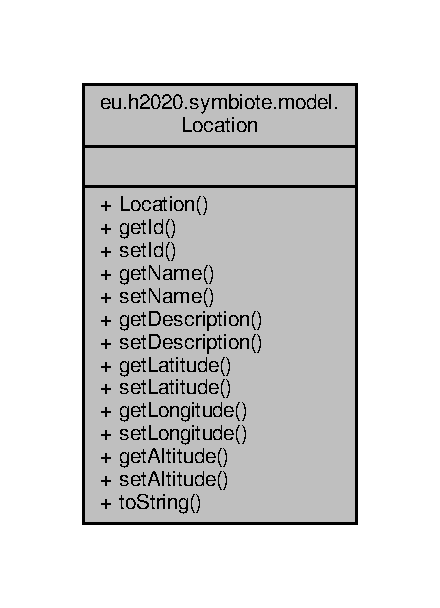
\includegraphics[width=211pt]{classeu_1_1h2020_1_1symbiote_1_1model_1_1Location__coll__graph}
\end{center}
\end{figure}
\subsection*{Public Member Functions}
\begin{DoxyCompactItemize}
\item 
\hyperlink{classeu_1_1h2020_1_1symbiote_1_1model_1_1Location_a49d03d727c3fecd9b3c618a2a6ed8abe}{Location} ()
\item 
String {\bfseries get\+Id} ()\hypertarget{classeu_1_1h2020_1_1symbiote_1_1model_1_1Location_a98a3b93d177deb7b9630c5e37547d80d}{}\label{classeu_1_1h2020_1_1symbiote_1_1model_1_1Location_a98a3b93d177deb7b9630c5e37547d80d}

\item 
void {\bfseries set\+Id} (String id)\hypertarget{classeu_1_1h2020_1_1symbiote_1_1model_1_1Location_a308f71eeeed57f22b5996da217028d29}{}\label{classeu_1_1h2020_1_1symbiote_1_1model_1_1Location_a308f71eeeed57f22b5996da217028d29}

\item 
String {\bfseries get\+Name} ()\hypertarget{classeu_1_1h2020_1_1symbiote_1_1model_1_1Location_a78e563a2622952f37da6f571932afa23}{}\label{classeu_1_1h2020_1_1symbiote_1_1model_1_1Location_a78e563a2622952f37da6f571932afa23}

\item 
void {\bfseries set\+Name} (String name)\hypertarget{classeu_1_1h2020_1_1symbiote_1_1model_1_1Location_a67ddf61270deeb669ebcdce9b9ead998}{}\label{classeu_1_1h2020_1_1symbiote_1_1model_1_1Location_a67ddf61270deeb669ebcdce9b9ead998}

\item 
String {\bfseries get\+Description} ()\hypertarget{classeu_1_1h2020_1_1symbiote_1_1model_1_1Location_accf0bb0ab10306a962e09fc32c8d821c}{}\label{classeu_1_1h2020_1_1symbiote_1_1model_1_1Location_accf0bb0ab10306a962e09fc32c8d821c}

\item 
void {\bfseries set\+Description} (String description)\hypertarget{classeu_1_1h2020_1_1symbiote_1_1model_1_1Location_a45d3f8f4397791af93669578501a43bf}{}\label{classeu_1_1h2020_1_1symbiote_1_1model_1_1Location_a45d3f8f4397791af93669578501a43bf}

\item 
double {\bfseries get\+Latitude} ()\hypertarget{classeu_1_1h2020_1_1symbiote_1_1model_1_1Location_a40812abe56323ccb3e65d1309d2d55e4}{}\label{classeu_1_1h2020_1_1symbiote_1_1model_1_1Location_a40812abe56323ccb3e65d1309d2d55e4}

\item 
void {\bfseries set\+Latitude} (double latitude)\hypertarget{classeu_1_1h2020_1_1symbiote_1_1model_1_1Location_a26b8aab258d4422bd5fc64d7a512b685}{}\label{classeu_1_1h2020_1_1symbiote_1_1model_1_1Location_a26b8aab258d4422bd5fc64d7a512b685}

\item 
double {\bfseries get\+Longitude} ()\hypertarget{classeu_1_1h2020_1_1symbiote_1_1model_1_1Location_afe9ac4993b9dbcc9350e2667e279d39b}{}\label{classeu_1_1h2020_1_1symbiote_1_1model_1_1Location_afe9ac4993b9dbcc9350e2667e279d39b}

\item 
void {\bfseries set\+Longitude} (double longitude)\hypertarget{classeu_1_1h2020_1_1symbiote_1_1model_1_1Location_a6bc9a04947915ea52001bccbcba0849e}{}\label{classeu_1_1h2020_1_1symbiote_1_1model_1_1Location_a6bc9a04947915ea52001bccbcba0849e}

\item 
double {\bfseries get\+Altitude} ()\hypertarget{classeu_1_1h2020_1_1symbiote_1_1model_1_1Location_a333c37abcd3c9ea766ca5ec6dddd5e3a}{}\label{classeu_1_1h2020_1_1symbiote_1_1model_1_1Location_a333c37abcd3c9ea766ca5ec6dddd5e3a}

\item 
void {\bfseries set\+Altitude} (double altitude)\hypertarget{classeu_1_1h2020_1_1symbiote_1_1model_1_1Location_ac2fc6d59229ad7253416f2fdf650675d}{}\label{classeu_1_1h2020_1_1symbiote_1_1model_1_1Location_ac2fc6d59229ad7253416f2fdf650675d}

\item 
String {\bfseries to\+String} ()\hypertarget{classeu_1_1h2020_1_1symbiote_1_1model_1_1Location_a5c3569ceefaa1d39a44d09fe8269abe6}{}\label{classeu_1_1h2020_1_1symbiote_1_1model_1_1Location_a5c3569ceefaa1d39a44d09fe8269abe6}

\end{DoxyCompactItemize}


\subsection{Detailed Description}
P\+O\+JO describing a location. 

\subsection{Constructor \& Destructor Documentation}
\index{eu\+::h2020\+::symbiote\+::model\+::\+Location@{eu\+::h2020\+::symbiote\+::model\+::\+Location}!Location@{Location}}
\index{Location@{Location}!eu\+::h2020\+::symbiote\+::model\+::\+Location@{eu\+::h2020\+::symbiote\+::model\+::\+Location}}
\subsubsection[{\texorpdfstring{Location()}{Location()}}]{\setlength{\rightskip}{0pt plus 5cm}eu.\+h2020.\+symbiote.\+model.\+Location.\+Location (
\begin{DoxyParamCaption}
{}
\end{DoxyParamCaption}
)}\hypertarget{classeu_1_1h2020_1_1symbiote_1_1model_1_1Location_a49d03d727c3fecd9b3c618a2a6ed8abe}{}\label{classeu_1_1h2020_1_1symbiote_1_1model_1_1Location_a49d03d727c3fecd9b3c618a2a6ed8abe}
Default empty constructor. 

The documentation for this class was generated from the following file\+:\begin{DoxyCompactItemize}
\item 
src/main/java/eu/h2020/symbiote/model/Location.\+java\end{DoxyCompactItemize}

\hypertarget{classeu_1_1h2020_1_1symbiote_1_1communication_1_1RabbitManager}{}\section{eu.\+h2020.\+symbiote.\+communication.\+Rabbit\+Manager Class Reference}
\label{classeu_1_1h2020_1_1symbiote_1_1communication_1_1RabbitManager}\index{eu.\+h2020.\+symbiote.\+communication.\+Rabbit\+Manager@{eu.\+h2020.\+symbiote.\+communication.\+Rabbit\+Manager}}


Collaboration diagram for eu.\+h2020.\+symbiote.\+communication.\+Rabbit\+Manager\+:
\nopagebreak
\begin{figure}[H]
\begin{center}
\leavevmode
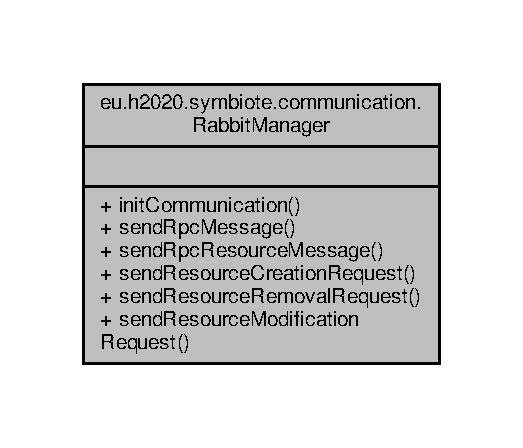
\includegraphics[width=250pt]{classeu_1_1h2020_1_1symbiote_1_1communication_1_1RabbitManager__coll__graph}
\end{center}
\end{figure}
\subsection*{Public Member Functions}
\begin{DoxyCompactItemize}
\item 
void \hyperlink{classeu_1_1h2020_1_1symbiote_1_1communication_1_1RabbitManager_a30abf6a670122eb22a8105a206858616}{init\+Communication} ()
\item 
String \hyperlink{classeu_1_1h2020_1_1symbiote_1_1communication_1_1RabbitManager_a822ebbed01755311ca9038bb7fa43591}{send\+Rpc\+Message} (String exchange\+Name, String routing\+Key, String message)
\item 
boolean \hyperlink{classeu_1_1h2020_1_1symbiote_1_1communication_1_1RabbitManager_aaf8fea1645c8e35ed2a1d8f8e2b4356f}{send\+Async\+Message} (String exchange\+Name, String routing\+Key, String message)
\item 
Core\+Resource\+Registry\+Response \hyperlink{classeu_1_1h2020_1_1symbiote_1_1communication_1_1RabbitManager_a98ca7f2122e2e4bb12d2252163177f0e}{send\+Rpc\+Resource\+Message} (String exchange\+Name, String routing\+Key, Core\+Resource\+Registry\+Request core\+Resource\+Request)
\item 
Core\+Resource\+Registry\+Response \hyperlink{classeu_1_1h2020_1_1symbiote_1_1communication_1_1RabbitManager_a4356c09360119574086e8c7ae7d7e676}{send\+Resource\+Creation\+Request} (Core\+Resource\+Registry\+Request core\+Resource\+Request)
\item 
Core\+Resource\+Registry\+Response \hyperlink{classeu_1_1h2020_1_1symbiote_1_1communication_1_1RabbitManager_a4ccbd77fad17957b8384cf53bf0af5e2}{send\+Resource\+Removal\+Request} (Core\+Resource\+Registry\+Request core\+Resource\+Request)
\item 
Core\+Resource\+Registry\+Response \hyperlink{classeu_1_1h2020_1_1symbiote_1_1communication_1_1RabbitManager_a2d8ecc7c67f2215a4e03dd082c6e39c0}{send\+Resource\+Modification\+Request} (Core\+Resource\+Registry\+Request core\+Resource\+Request)
\item 
boolean \hyperlink{classeu_1_1h2020_1_1symbiote_1_1communication_1_1RabbitManager_a18b771d2db6a06469a6776ebf0ff96e1}{send\+Monitoring\+Message} (Cloud\+Monitoring\+Platform cloud\+Monitoring\+Platform)
\end{DoxyCompactItemize}


\subsection{Detailed Description}
Class used for all internal communication using Rabbit\+MQ A\+M\+QP implementation. It works as a Spring Bean, and should be used via autowiring. 

\hyperlink{classeu_1_1h2020_1_1symbiote_1_1communication_1_1RabbitManager}{Rabbit\+Manager} uses properties taken from Core\+Config\+Server to set up communication (exchange parameters, routing keys etc.) 

\subsection{Member Function Documentation}
\mbox{\Hypertarget{classeu_1_1h2020_1_1symbiote_1_1communication_1_1RabbitManager_a30abf6a670122eb22a8105a206858616}\label{classeu_1_1h2020_1_1symbiote_1_1communication_1_1RabbitManager_a30abf6a670122eb22a8105a206858616}} 
\index{eu\+::h2020\+::symbiote\+::communication\+::\+Rabbit\+Manager@{eu\+::h2020\+::symbiote\+::communication\+::\+Rabbit\+Manager}!init\+Communication@{init\+Communication}}
\index{init\+Communication@{init\+Communication}!eu\+::h2020\+::symbiote\+::communication\+::\+Rabbit\+Manager@{eu\+::h2020\+::symbiote\+::communication\+::\+Rabbit\+Manager}}
\subsubsection{\texorpdfstring{init\+Communication()}{initCommunication()}}
{\footnotesize\ttfamily void eu.\+h2020.\+symbiote.\+communication.\+Rabbit\+Manager.\+init\+Communication (\begin{DoxyParamCaption}{ }\end{DoxyParamCaption})}

Method used to initialise Rabbit\+MQ connection and declare all required exchanges. This method should be called once, after bean initialization (so that properties from Core\+Config\+Server are obtained), but before using \hyperlink{classeu_1_1h2020_1_1symbiote_1_1communication_1_1RabbitManager}{Rabbit\+Manager} to send any message. \mbox{\Hypertarget{classeu_1_1h2020_1_1symbiote_1_1communication_1_1RabbitManager_aaf8fea1645c8e35ed2a1d8f8e2b4356f}\label{classeu_1_1h2020_1_1symbiote_1_1communication_1_1RabbitManager_aaf8fea1645c8e35ed2a1d8f8e2b4356f}} 
\index{eu\+::h2020\+::symbiote\+::communication\+::\+Rabbit\+Manager@{eu\+::h2020\+::symbiote\+::communication\+::\+Rabbit\+Manager}!send\+Async\+Message@{send\+Async\+Message}}
\index{send\+Async\+Message@{send\+Async\+Message}!eu\+::h2020\+::symbiote\+::communication\+::\+Rabbit\+Manager@{eu\+::h2020\+::symbiote\+::communication\+::\+Rabbit\+Manager}}
\subsubsection{\texorpdfstring{send\+Async\+Message()}{sendAsyncMessage()}}
{\footnotesize\ttfamily boolean eu.\+h2020.\+symbiote.\+communication.\+Rabbit\+Manager.\+send\+Async\+Message (\begin{DoxyParamCaption}\item[{String}]{exchange\+Name,  }\item[{String}]{routing\+Key,  }\item[{String}]{message }\end{DoxyParamCaption})}

Method used to send an asynchronous message, without expecting any returning result. Exchange should be declared before sending the message.


\begin{DoxyParams}{Parameters}
{\em exchange\+Name} & name of the exchange to send message to \\
\hline
{\em routing\+Key} & routing key to send message to \\
\hline
{\em message} & message to be sent \\
\hline
\end{DoxyParams}
\begin{DoxyReturn}{Returns}
true if publish went ok, false otherwise 
\end{DoxyReturn}
\mbox{\Hypertarget{classeu_1_1h2020_1_1symbiote_1_1communication_1_1RabbitManager_a18b771d2db6a06469a6776ebf0ff96e1}\label{classeu_1_1h2020_1_1symbiote_1_1communication_1_1RabbitManager_a18b771d2db6a06469a6776ebf0ff96e1}} 
\index{eu\+::h2020\+::symbiote\+::communication\+::\+Rabbit\+Manager@{eu\+::h2020\+::symbiote\+::communication\+::\+Rabbit\+Manager}!send\+Monitoring\+Message@{send\+Monitoring\+Message}}
\index{send\+Monitoring\+Message@{send\+Monitoring\+Message}!eu\+::h2020\+::symbiote\+::communication\+::\+Rabbit\+Manager@{eu\+::h2020\+::symbiote\+::communication\+::\+Rabbit\+Manager}}
\subsubsection{\texorpdfstring{send\+Monitoring\+Message()}{sendMonitoringMessage()}}
{\footnotesize\ttfamily boolean eu.\+h2020.\+symbiote.\+communication.\+Rabbit\+Manager.\+send\+Monitoring\+Message (\begin{DoxyParamCaption}\item[{Cloud\+Monitoring\+Platform}]{cloud\+Monitoring\+Platform }\end{DoxyParamCaption})}

Method used to send asynchronous, monitoring message to Core Resource Monitor.


\begin{DoxyParams}{Parameters}
{\em cloud\+Monitoring\+Platform} & message from platform \\
\hline
\end{DoxyParams}
\begin{DoxyReturn}{Returns}
true if message is sent ok, false otherwise 
\end{DoxyReturn}
\mbox{\Hypertarget{classeu_1_1h2020_1_1symbiote_1_1communication_1_1RabbitManager_a4356c09360119574086e8c7ae7d7e676}\label{classeu_1_1h2020_1_1symbiote_1_1communication_1_1RabbitManager_a4356c09360119574086e8c7ae7d7e676}} 
\index{eu\+::h2020\+::symbiote\+::communication\+::\+Rabbit\+Manager@{eu\+::h2020\+::symbiote\+::communication\+::\+Rabbit\+Manager}!send\+Resource\+Creation\+Request@{send\+Resource\+Creation\+Request}}
\index{send\+Resource\+Creation\+Request@{send\+Resource\+Creation\+Request}!eu\+::h2020\+::symbiote\+::communication\+::\+Rabbit\+Manager@{eu\+::h2020\+::symbiote\+::communication\+::\+Rabbit\+Manager}}
\subsubsection{\texorpdfstring{send\+Resource\+Creation\+Request()}{sendResourceCreationRequest()}}
{\footnotesize\ttfamily Core\+Resource\+Registry\+Response eu.\+h2020.\+symbiote.\+communication.\+Rabbit\+Manager.\+send\+Resource\+Creation\+Request (\begin{DoxyParamCaption}\item[{Core\+Resource\+Registry\+Request}]{core\+Resource\+Request }\end{DoxyParamCaption})}

Method used to send R\+PC request to create resource.


\begin{DoxyParams}{Parameters}
{\em core\+Resource\+Request} & resource to be created \\
\hline
\end{DoxyParams}
\begin{DoxyReturn}{Returns}
object containing status of requested operation and, if successful, a resource object containing assigned ID 
\end{DoxyReturn}
\mbox{\Hypertarget{classeu_1_1h2020_1_1symbiote_1_1communication_1_1RabbitManager_a2d8ecc7c67f2215a4e03dd082c6e39c0}\label{classeu_1_1h2020_1_1symbiote_1_1communication_1_1RabbitManager_a2d8ecc7c67f2215a4e03dd082c6e39c0}} 
\index{eu\+::h2020\+::symbiote\+::communication\+::\+Rabbit\+Manager@{eu\+::h2020\+::symbiote\+::communication\+::\+Rabbit\+Manager}!send\+Resource\+Modification\+Request@{send\+Resource\+Modification\+Request}}
\index{send\+Resource\+Modification\+Request@{send\+Resource\+Modification\+Request}!eu\+::h2020\+::symbiote\+::communication\+::\+Rabbit\+Manager@{eu\+::h2020\+::symbiote\+::communication\+::\+Rabbit\+Manager}}
\subsubsection{\texorpdfstring{send\+Resource\+Modification\+Request()}{sendResourceModificationRequest()}}
{\footnotesize\ttfamily Core\+Resource\+Registry\+Response eu.\+h2020.\+symbiote.\+communication.\+Rabbit\+Manager.\+send\+Resource\+Modification\+Request (\begin{DoxyParamCaption}\item[{Core\+Resource\+Registry\+Request}]{core\+Resource\+Request }\end{DoxyParamCaption})}

Method used to send R\+PC request to modify resource.


\begin{DoxyParams}{Parameters}
{\em core\+Resource\+Request} & resource to be modified \\
\hline
\end{DoxyParams}
\begin{DoxyReturn}{Returns}
object containing status of requested operation and, if successful, a resource object 
\end{DoxyReturn}
\mbox{\Hypertarget{classeu_1_1h2020_1_1symbiote_1_1communication_1_1RabbitManager_a4ccbd77fad17957b8384cf53bf0af5e2}\label{classeu_1_1h2020_1_1symbiote_1_1communication_1_1RabbitManager_a4ccbd77fad17957b8384cf53bf0af5e2}} 
\index{eu\+::h2020\+::symbiote\+::communication\+::\+Rabbit\+Manager@{eu\+::h2020\+::symbiote\+::communication\+::\+Rabbit\+Manager}!send\+Resource\+Removal\+Request@{send\+Resource\+Removal\+Request}}
\index{send\+Resource\+Removal\+Request@{send\+Resource\+Removal\+Request}!eu\+::h2020\+::symbiote\+::communication\+::\+Rabbit\+Manager@{eu\+::h2020\+::symbiote\+::communication\+::\+Rabbit\+Manager}}
\subsubsection{\texorpdfstring{send\+Resource\+Removal\+Request()}{sendResourceRemovalRequest()}}
{\footnotesize\ttfamily Core\+Resource\+Registry\+Response eu.\+h2020.\+symbiote.\+communication.\+Rabbit\+Manager.\+send\+Resource\+Removal\+Request (\begin{DoxyParamCaption}\item[{Core\+Resource\+Registry\+Request}]{core\+Resource\+Request }\end{DoxyParamCaption})}

Method used to send R\+PC request to remove resource.


\begin{DoxyParams}{Parameters}
{\em core\+Resource\+Request} & resource to be removed \\
\hline
\end{DoxyParams}
\begin{DoxyReturn}{Returns}
object containing status of requested operation and, if successful, a resource object 
\end{DoxyReturn}
\mbox{\Hypertarget{classeu_1_1h2020_1_1symbiote_1_1communication_1_1RabbitManager_a822ebbed01755311ca9038bb7fa43591}\label{classeu_1_1h2020_1_1symbiote_1_1communication_1_1RabbitManager_a822ebbed01755311ca9038bb7fa43591}} 
\index{eu\+::h2020\+::symbiote\+::communication\+::\+Rabbit\+Manager@{eu\+::h2020\+::symbiote\+::communication\+::\+Rabbit\+Manager}!send\+Rpc\+Message@{send\+Rpc\+Message}}
\index{send\+Rpc\+Message@{send\+Rpc\+Message}!eu\+::h2020\+::symbiote\+::communication\+::\+Rabbit\+Manager@{eu\+::h2020\+::symbiote\+::communication\+::\+Rabbit\+Manager}}
\subsubsection{\texorpdfstring{send\+Rpc\+Message()}{sendRpcMessage()}}
{\footnotesize\ttfamily String eu.\+h2020.\+symbiote.\+communication.\+Rabbit\+Manager.\+send\+Rpc\+Message (\begin{DoxyParamCaption}\item[{String}]{exchange\+Name,  }\item[{String}]{routing\+Key,  }\item[{String}]{message }\end{DoxyParamCaption})}

Method used to send message via R\+PC (Remote Procedure Call) pattern. In this implementation it covers asynchronous Rabbit communication with synchronous one, as it is used by conventional R\+E\+ST facade. Before sending a message, a temporary response queue is declared and its name is passed along with the message. When a consumer handles the message, it returns the result via the response queue. Since this is a synchronous pattern, it uses timeout of 20 seconds. If the response doesn\textquotesingle{}t come in that time, the method returns with null result.


\begin{DoxyParams}{Parameters}
{\em exchange\+Name} & name of the exchange to send message to \\
\hline
{\em routing\+Key} & routing key to send message to \\
\hline
{\em message} & message to be sent \\
\hline
\end{DoxyParams}
\begin{DoxyReturn}{Returns}
response from the consumer or null if timeout occurs 
\end{DoxyReturn}
\mbox{\Hypertarget{classeu_1_1h2020_1_1symbiote_1_1communication_1_1RabbitManager_a98ca7f2122e2e4bb12d2252163177f0e}\label{classeu_1_1h2020_1_1symbiote_1_1communication_1_1RabbitManager_a98ca7f2122e2e4bb12d2252163177f0e}} 
\index{eu\+::h2020\+::symbiote\+::communication\+::\+Rabbit\+Manager@{eu\+::h2020\+::symbiote\+::communication\+::\+Rabbit\+Manager}!send\+Rpc\+Resource\+Message@{send\+Rpc\+Resource\+Message}}
\index{send\+Rpc\+Resource\+Message@{send\+Rpc\+Resource\+Message}!eu\+::h2020\+::symbiote\+::communication\+::\+Rabbit\+Manager@{eu\+::h2020\+::symbiote\+::communication\+::\+Rabbit\+Manager}}
\subsubsection{\texorpdfstring{send\+Rpc\+Resource\+Message()}{sendRpcResourceMessage()}}
{\footnotesize\ttfamily Core\+Resource\+Registry\+Response eu.\+h2020.\+symbiote.\+communication.\+Rabbit\+Manager.\+send\+Rpc\+Resource\+Message (\begin{DoxyParamCaption}\item[{String}]{exchange\+Name,  }\item[{String}]{routing\+Key,  }\item[{Core\+Resource\+Registry\+Request}]{core\+Resource\+Request }\end{DoxyParamCaption})}

Helper method that provides J\+S\+ON marshalling and unmarshalling for the sake of Rabbit communication.


\begin{DoxyParams}{Parameters}
{\em exchange\+Name} & name of the exchange to send message to \\
\hline
{\em routing\+Key} & routing key to send message to \\
\hline
{\em core\+Resource\+Request} & resource to be sent \\
\hline
\end{DoxyParams}
\begin{DoxyReturn}{Returns}
response from the consumer or null if timeout occurs 
\end{DoxyReturn}


The documentation for this class was generated from the following file\+:\begin{DoxyCompactItemize}
\item 
src/main/java/eu/h2020/symbiote/communication/Rabbit\+Manager.\+java\end{DoxyCompactItemize}

\hypertarget{classeu_1_1h2020_1_1symbiote_1_1model_1_1Resource}{}\section{eu.\+h2020.\+symbiote.\+model.\+Resource Class Reference}
\label{classeu_1_1h2020_1_1symbiote_1_1model_1_1Resource}\index{eu.\+h2020.\+symbiote.\+model.\+Resource@{eu.\+h2020.\+symbiote.\+model.\+Resource}}


Collaboration diagram for eu.\+h2020.\+symbiote.\+model.\+Resource\+:
\nopagebreak
\begin{figure}[H]
\begin{center}
\leavevmode
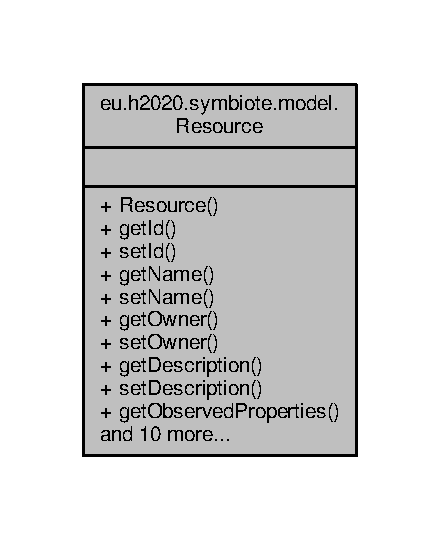
\includegraphics[width=211pt]{classeu_1_1h2020_1_1symbiote_1_1model_1_1Resource__coll__graph}
\end{center}
\end{figure}
\subsection*{Public Member Functions}
\begin{DoxyCompactItemize}
\item 
\hyperlink{classeu_1_1h2020_1_1symbiote_1_1model_1_1Resource_a18db6b9a6779a00b03f700b26bf7840b}{Resource} ()
\item 
String {\bfseries get\+Id} ()\hypertarget{classeu_1_1h2020_1_1symbiote_1_1model_1_1Resource_a6d2b00f0e94b55cce1daff002012369c}{}\label{classeu_1_1h2020_1_1symbiote_1_1model_1_1Resource_a6d2b00f0e94b55cce1daff002012369c}

\item 
void {\bfseries set\+Id} (String id)\hypertarget{classeu_1_1h2020_1_1symbiote_1_1model_1_1Resource_a209815ba7cdb6b82334e664eb4c38708}{}\label{classeu_1_1h2020_1_1symbiote_1_1model_1_1Resource_a209815ba7cdb6b82334e664eb4c38708}

\item 
String {\bfseries get\+Name} ()\hypertarget{classeu_1_1h2020_1_1symbiote_1_1model_1_1Resource_a7332986d4dfa4ca233f705659f166f2c}{}\label{classeu_1_1h2020_1_1symbiote_1_1model_1_1Resource_a7332986d4dfa4ca233f705659f166f2c}

\item 
void {\bfseries set\+Name} (String name)\hypertarget{classeu_1_1h2020_1_1symbiote_1_1model_1_1Resource_ad2cd06bcbfa928adead9017509cc2e78}{}\label{classeu_1_1h2020_1_1symbiote_1_1model_1_1Resource_ad2cd06bcbfa928adead9017509cc2e78}

\item 
String {\bfseries get\+Owner} ()\hypertarget{classeu_1_1h2020_1_1symbiote_1_1model_1_1Resource_a0bd495e4c9a10fac6e885de268b5ad76}{}\label{classeu_1_1h2020_1_1symbiote_1_1model_1_1Resource_a0bd495e4c9a10fac6e885de268b5ad76}

\item 
void {\bfseries set\+Owner} (String owner)\hypertarget{classeu_1_1h2020_1_1symbiote_1_1model_1_1Resource_a4391365a9ef765fb9c96e8243a45fafb}{}\label{classeu_1_1h2020_1_1symbiote_1_1model_1_1Resource_a4391365a9ef765fb9c96e8243a45fafb}

\item 
String {\bfseries get\+Description} ()\hypertarget{classeu_1_1h2020_1_1symbiote_1_1model_1_1Resource_ae2ce583e094c18bca236027602739049}{}\label{classeu_1_1h2020_1_1symbiote_1_1model_1_1Resource_ae2ce583e094c18bca236027602739049}

\item 
void {\bfseries set\+Description} (String description)\hypertarget{classeu_1_1h2020_1_1symbiote_1_1model_1_1Resource_a19349909b51f43be943fcc3ebc078009}{}\label{classeu_1_1h2020_1_1symbiote_1_1model_1_1Resource_a19349909b51f43be943fcc3ebc078009}

\item 
List$<$ String $>$ {\bfseries get\+Observed\+Properties} ()\hypertarget{classeu_1_1h2020_1_1symbiote_1_1model_1_1Resource_a2aaf59e1be5b0c974a31e106adfa6c43}{}\label{classeu_1_1h2020_1_1symbiote_1_1model_1_1Resource_a2aaf59e1be5b0c974a31e106adfa6c43}

\item 
void {\bfseries set\+Observed\+Properties} (List$<$ String $>$ observed\+Properties)\hypertarget{classeu_1_1h2020_1_1symbiote_1_1model_1_1Resource_a826dbee60cf539ffbf1a088496ac7e11}{}\label{classeu_1_1h2020_1_1symbiote_1_1model_1_1Resource_a826dbee60cf539ffbf1a088496ac7e11}

\item 
String {\bfseries get\+Resource\+U\+RL} ()\hypertarget{classeu_1_1h2020_1_1symbiote_1_1model_1_1Resource_a4a0c05d9007f2216c55ddc32a44f467b}{}\label{classeu_1_1h2020_1_1symbiote_1_1model_1_1Resource_a4a0c05d9007f2216c55ddc32a44f467b}

\item 
void {\bfseries set\+Resource\+U\+RL} (String resource\+U\+RL)\hypertarget{classeu_1_1h2020_1_1symbiote_1_1model_1_1Resource_a27d7401a8087bf902fd575039d574d0c}{}\label{classeu_1_1h2020_1_1symbiote_1_1model_1_1Resource_a27d7401a8087bf902fd575039d574d0c}

\item 
\hyperlink{classeu_1_1h2020_1_1symbiote_1_1model_1_1Location}{Location} {\bfseries get\+Location} ()\hypertarget{classeu_1_1h2020_1_1symbiote_1_1model_1_1Resource_acfb7ead093f1ed692640c99daba8fc6c}{}\label{classeu_1_1h2020_1_1symbiote_1_1model_1_1Resource_acfb7ead093f1ed692640c99daba8fc6c}

\item 
void {\bfseries set\+Location} (\hyperlink{classeu_1_1h2020_1_1symbiote_1_1model_1_1Location}{Location} location)\hypertarget{classeu_1_1h2020_1_1symbiote_1_1model_1_1Resource_a14eba3bd0171783f32d6d4446768905d}{}\label{classeu_1_1h2020_1_1symbiote_1_1model_1_1Resource_a14eba3bd0171783f32d6d4446768905d}

\item 
String {\bfseries get\+Feature\+Of\+Interest} ()\hypertarget{classeu_1_1h2020_1_1symbiote_1_1model_1_1Resource_a1e5912a2e60f0d2dcda674f26ebe871b}{}\label{classeu_1_1h2020_1_1symbiote_1_1model_1_1Resource_a1e5912a2e60f0d2dcda674f26ebe871b}

\item 
void {\bfseries set\+Feature\+Of\+Interest} (String feature\+Of\+Interest)\hypertarget{classeu_1_1h2020_1_1symbiote_1_1model_1_1Resource_abcfd5b3b2e1515ca7e9eb50eeb7ed0cf}{}\label{classeu_1_1h2020_1_1symbiote_1_1model_1_1Resource_abcfd5b3b2e1515ca7e9eb50eeb7ed0cf}

\item 
String {\bfseries get\+Platform\+Id} ()\hypertarget{classeu_1_1h2020_1_1symbiote_1_1model_1_1Resource_a97e847fb787ea9fe1d16d8bd702deece}{}\label{classeu_1_1h2020_1_1symbiote_1_1model_1_1Resource_a97e847fb787ea9fe1d16d8bd702deece}

\item 
void {\bfseries set\+Platform\+Id} (String platform\+Id)\hypertarget{classeu_1_1h2020_1_1symbiote_1_1model_1_1Resource_a4f3c37b066d6e6587912fa1f1240048f}{}\label{classeu_1_1h2020_1_1symbiote_1_1model_1_1Resource_a4f3c37b066d6e6587912fa1f1240048f}

\item 
String {\bfseries to\+String} ()\hypertarget{classeu_1_1h2020_1_1symbiote_1_1model_1_1Resource_a2268176e848f8301d5fd04c71899ec91}{}\label{classeu_1_1h2020_1_1symbiote_1_1model_1_1Resource_a2268176e848f8301d5fd04c71899ec91}

\end{DoxyCompactItemize}


\subsection{Detailed Description}
P\+O\+JO describing a resource. 

\subsection{Constructor \& Destructor Documentation}
\index{eu\+::h2020\+::symbiote\+::model\+::\+Resource@{eu\+::h2020\+::symbiote\+::model\+::\+Resource}!Resource@{Resource}}
\index{Resource@{Resource}!eu\+::h2020\+::symbiote\+::model\+::\+Resource@{eu\+::h2020\+::symbiote\+::model\+::\+Resource}}
\subsubsection[{\texorpdfstring{Resource()}{Resource()}}]{\setlength{\rightskip}{0pt plus 5cm}eu.\+h2020.\+symbiote.\+model.\+Resource.\+Resource (
\begin{DoxyParamCaption}
{}
\end{DoxyParamCaption}
)}\hypertarget{classeu_1_1h2020_1_1symbiote_1_1model_1_1Resource_a18db6b9a6779a00b03f700b26bf7840b}{}\label{classeu_1_1h2020_1_1symbiote_1_1model_1_1Resource_a18db6b9a6779a00b03f700b26bf7840b}
Default empty constructor. 

The documentation for this class was generated from the following file\+:\begin{DoxyCompactItemize}
\item 
src/main/java/eu/h2020/symbiote/model/Resource.\+java\end{DoxyCompactItemize}

\hypertarget{classeu_1_1h2020_1_1symbiote_1_1model_1_1RpcResourceResponse}{}\section{eu.\+h2020.\+symbiote.\+model.\+Rpc\+Resource\+Response Class Reference}
\label{classeu_1_1h2020_1_1symbiote_1_1model_1_1RpcResourceResponse}\index{eu.\+h2020.\+symbiote.\+model.\+Rpc\+Resource\+Response@{eu.\+h2020.\+symbiote.\+model.\+Rpc\+Resource\+Response}}


Collaboration diagram for eu.\+h2020.\+symbiote.\+model.\+Rpc\+Resource\+Response\+:
\nopagebreak
\begin{figure}[H]
\begin{center}
\leavevmode
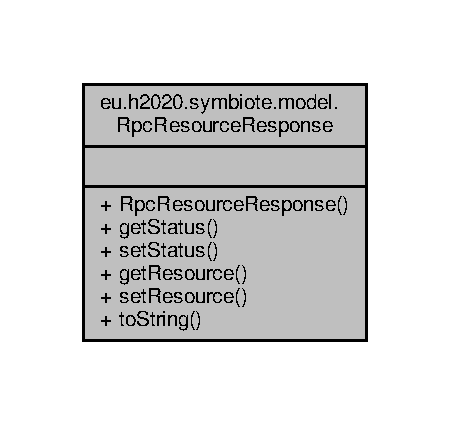
\includegraphics[width=216pt]{classeu_1_1h2020_1_1symbiote_1_1model_1_1RpcResourceResponse__coll__graph}
\end{center}
\end{figure}
\subsection*{Public Member Functions}
\begin{DoxyCompactItemize}
\item 
\hyperlink{classeu_1_1h2020_1_1symbiote_1_1model_1_1RpcResourceResponse_aa3fb7986c653ddbe97463011290fe2a7}{Rpc\+Resource\+Response} ()
\item 
int {\bfseries get\+Status} ()\hypertarget{classeu_1_1h2020_1_1symbiote_1_1model_1_1RpcResourceResponse_a64655e4dbe4ba990cc6db5c963c5f2b7}{}\label{classeu_1_1h2020_1_1symbiote_1_1model_1_1RpcResourceResponse_a64655e4dbe4ba990cc6db5c963c5f2b7}

\item 
void {\bfseries set\+Status} (int status)\hypertarget{classeu_1_1h2020_1_1symbiote_1_1model_1_1RpcResourceResponse_aa02fb9113fa7af9d2b2bd980d08a7571}{}\label{classeu_1_1h2020_1_1symbiote_1_1model_1_1RpcResourceResponse_aa02fb9113fa7af9d2b2bd980d08a7571}

\item 
\hyperlink{classeu_1_1h2020_1_1symbiote_1_1model_1_1Resource}{Resource} {\bfseries get\+Resource} ()\hypertarget{classeu_1_1h2020_1_1symbiote_1_1model_1_1RpcResourceResponse_adfbf0e5849dc241586d264bef8aa19f6}{}\label{classeu_1_1h2020_1_1symbiote_1_1model_1_1RpcResourceResponse_adfbf0e5849dc241586d264bef8aa19f6}

\item 
void {\bfseries set\+Resource} (\hyperlink{classeu_1_1h2020_1_1symbiote_1_1model_1_1Resource}{Resource} resource)\hypertarget{classeu_1_1h2020_1_1symbiote_1_1model_1_1RpcResourceResponse_a4700ed3c58d3cac28ba62da378ae002e}{}\label{classeu_1_1h2020_1_1symbiote_1_1model_1_1RpcResourceResponse_a4700ed3c58d3cac28ba62da378ae002e}

\item 
String {\bfseries to\+String} ()\hypertarget{classeu_1_1h2020_1_1symbiote_1_1model_1_1RpcResourceResponse_a5caff9d21a27972951f087f17ad24da7}{}\label{classeu_1_1h2020_1_1symbiote_1_1model_1_1RpcResourceResponse_a5caff9d21a27972951f087f17ad24da7}

\end{DoxyCompactItemize}


\subsection{Detailed Description}
Class used as a response to R\+PC call requesting resource operation 

\subsection{Constructor \& Destructor Documentation}
\index{eu\+::h2020\+::symbiote\+::model\+::\+Rpc\+Resource\+Response@{eu\+::h2020\+::symbiote\+::model\+::\+Rpc\+Resource\+Response}!Rpc\+Resource\+Response@{Rpc\+Resource\+Response}}
\index{Rpc\+Resource\+Response@{Rpc\+Resource\+Response}!eu\+::h2020\+::symbiote\+::model\+::\+Rpc\+Resource\+Response@{eu\+::h2020\+::symbiote\+::model\+::\+Rpc\+Resource\+Response}}
\subsubsection[{\texorpdfstring{Rpc\+Resource\+Response()}{RpcResourceResponse()}}]{\setlength{\rightskip}{0pt plus 5cm}eu.\+h2020.\+symbiote.\+model.\+Rpc\+Resource\+Response.\+Rpc\+Resource\+Response (
\begin{DoxyParamCaption}
{}
\end{DoxyParamCaption}
)}\hypertarget{classeu_1_1h2020_1_1symbiote_1_1model_1_1RpcResourceResponse_aa3fb7986c653ddbe97463011290fe2a7}{}\label{classeu_1_1h2020_1_1symbiote_1_1model_1_1RpcResourceResponse_aa3fb7986c653ddbe97463011290fe2a7}
Default empty constructor. 

The documentation for this class was generated from the following file\+:\begin{DoxyCompactItemize}
\item 
src/main/java/eu/h2020/symbiote/model/Rpc\+Resource\+Response.\+java\end{DoxyCompactItemize}

%--- End generated contents ---

% Index
\backmatter
\newpage
\phantomsection
\clearemptydoublepage
\addcontentsline{toc}{chapter}{Index}
\printindex

\end{document}
